\section{Equações do Movimento Orbital e Manobras Orbitais Associadas ao Problema de RVD/B - Dinâmica Orbital}

O problema dos dois corpos, proposto por Isaac Newton \cite{newton1713}, consiste em determinar as posições e velocidades de duas partículas em qualquer instante de tempo, desde que sejam conhecidas as suas posições, massas e velocidades em um dado instante $t$, e que ambas as partículas se movam sob a ação de sua força de gravidade mútua.  
Como exemplo prático do problema dos dois corpos, pode-se citar a órbita da Lua em torno da Terra, bem como a de um planeta em torno do Sol \cite{wgsantos2011}.
A aceleração de cada corpo é dada por:

\begin{equation}
\label{eq:aceleracao_Corpo1}
m_1 \ddot{\vec R}_1 =
+ G \frac{m_1m_2}{r^2} \frac{\vect r}{r} =
+ G \frac{m_1m_2}{r^3} {\vect r}
\end{equation}

\begin{equation}
\label{eq:aceleracao_Corpo2}
m_2 \ddot{\vec R}_2 =
- G \frac{m_1m_2}{r^2} \frac{\vect r}{r} =
- G \frac{m_1m_2}{r^3} {\vect r}
\end{equation}

Onde:
\begin{equation}
    \label{eq:vetor_posicao_r}
\vect{r} = \vec R_{\, 2} - \vec R_{\, 1}
\end{equation}

\begin{figure}[ht]
    \centering
    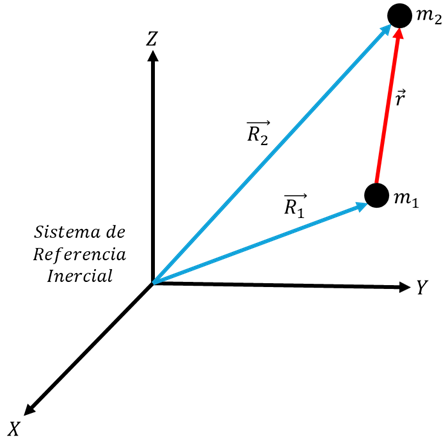
\includegraphics[width=0.5\textwidth]{2 Formulacao do problema/Imagens/Problema dos dois corpos.png}
    \caption{Problema dos dois corpos. Fonte: Adaptado de Bong Wie (2008).}
    \label{fig:problema_doisCorpos}
\end{figure}

A equação \eqref{eq:vetor_posicao_r} é o vetor posição de $m_2$ em relação a $m_1$ e em relação ao centro da Terra \cite{wie2008space}; e, $r$ é a distância entre um corpo em relação ao outro. Portanto, somando as equações \eqref{eq:aceleracao_Corpo1} e \eqref{eq:aceleracao_Corpo2}, obtém-se:

\begin{equation}
\label{eq:somaAceleracao_Corpo1e2}
m_1 \ddot{\vec R}_1 + m_2 \ddot{\vec R}_2 = 0
\end{equation}

A partir da Lei da Gravitação Universal, equação \eqref{eq:newtonGravitacao_Parte1}, o termo $G M$ é denominado parâmetro gravitacional ($\mu$ da Terra), onde $M$ representa a massa da Terra; $m_1$ e $m_2$ são as massas dos corpos (\textit{chaser} e \textit{target}, respectivamente); $G = 6,6695 \times 10^{-11}$ é a constante gravitacional \cite{halliday2013,wie2008space}.

\begin{equation}
\label{eq:newtonGravitacao_Parte1}
\vect F_g(\vect r) = - G\ \frac{M(m_1+m_2)}{r^2} \frac{\vect r}{r} = - G\ \frac{M(m_1+m_2)}{r^3} {\vect r}
\end{equation}

Na maioria dos casos práticos de mecânica orbital, a massa do corpo primário ($M$) — neste caso, a massa do planeta Terra — é muito maior que a do corpo secundário ($m_1$ e $m_2$), então essas massas menores podem ser ignoradas \cite{Folta2022}, desta forma, $M \gg (m_1 + m_2)$, e que resulta em $\mu \approx GM$ \cite{wie2008space}. Dito isso, a equação do movimento orbital sob a ação da gravidade é dada por \cite{newton1713}:

\begin{equation}
\label{eq:newtonGravitacao_Parte2}
\vect F_g(\vect r) = - G\ \frac{Mm}{r^2} {\vect r}
\end{equation}
 
\begin{equation}
\label{eq:fgParte1}
\vect F_g(\vect r) = -\mu \frac{m}{\vec {r^3}} \vect r
\end{equation}

\begin{equation}
\label{eq:fgParte2}
\frac{\vect F_g(\vect r)}{m} = -\mu \frac{\vect r}{\vec {r^3}}
\end{equation}

Pela segunda Lei de Newton \cite{newton1713}, a força é o produto da massa pela aceleração \cite{halliday2013} - que é o mesmo que a derivada segunda da posição em relação ao tempo \cite{edelstein2018_derivadaSegunda}.

\begin{equation}
\label{eq:F=ma_Halliday2013Parte1}
\vect F_g(\vect r) = m * \vec a = m * \ddot{\vect r}
\end{equation}

\begin{equation}
\label{eq:Fma_Halliday2013_Parte2}
\frac{\vect F_g(\vect r)}{m} = \ddot{\vect r}
\end{equation}

Substituíndo a equação \eqref{eq:Fma_Halliday2013_Parte2} na equação \eqref{eq:fgParte2}:

\begin{equation}
\label{eq:eqFundamentalDoisCorpos}
\ddot {\vect r} = -\mu \frac{\vec r}{\vec {r^3}}
\end{equation}

Onde $\ddot{\vect r}$ é a aceleração inercial de $m_2$ em relação a $m_1$; $\mu$ é o parâmetro gravitacional do sistema de dois corpos, e \eqref{eq:eqFundamentalDoisCorpos} é a equação fundamental (geral) do problema dos dois corpos \cite{fehse2003,wie2008space}

% Para o \emph{target}, a equação do movimento é dado por:

% \begin{equation}
% \label{eq:movimentoTarget}
% \ddot{\vect r_t} = -\mu \frac{\vect r_t}{\vect r_t ^{3}}
% \end{equation}

% Enquanto que a equação do movimento para o \emph{chaser}, é dada por:

% \begin{equation}
% \label{eq:movimentoChaser}
% \ddot{\vect r_c} = -\mu \frac{\vect r_c}{\vect r_c ^{3}} + \frac{\vect F}{m_c}
% \end{equation}

O \emph{target} (não-propulsado) obedece:
\begin{equation}
\label{eq:movimentoTarget}
\ddot{\vec r_t} = -\,\mu\,\frac{\vec {r_t^3}}{\vec {r^3}}\,.
\end{equation}

Enquanto que o \emph{chaser} (com força de controle) obedece:
\begin{equation}
\label{eq:movimentoChaser}
\ddot{\vec r_c} = -\,\mu\,\frac{\vec r_c}{\vec {r_c^3}} \;+\; \frac{\vec F}{m_c}\,,
\end{equation}
onde \(\vec F\) é a força (controle) aplicada.
